\documentclass[a4paper,fleqn,12pt]{article}

\usepackage[utf8]{inputenc}
\usepackage[bulgarian]{babel}
\usepackage{amsmath}
\usepackage{amssymb}
\usepackage{booktabs}
\usepackage{fancyhdr}
\usepackage{amsthm}
\usepackage{graphicx}

\theoremstyle{definition}
\newtheorem{theorem}{Tеорема}[subsection]
\newtheorem{lemma}[theorem]{Лема}

\newtheorem{definition}{Дефиниция}[subsection]

\newtheorem{example}{Пример}[subsection]

\newtheorem{task}{Задача}[subsection]



\title{Математически анализ 2 \\ Упражнения}
\author{Exonaut}

\pagestyle{fancy}
\fancyhf{}
\lhead{\rightmark}
\rhead{\thepage}
\cfoot{}
\renewcommand{\headrulewidth}{0pt}

\begin{document}

\pagenumbering{gobble}
\maketitle

\newpage
\pagenumbering{arabic}

\tableofcontents
\newpage

\section{Упражнение към лекция 1}
\subsection{Задачи}

\subsection*{Задача 1}
Да се покаже дали посочените редици $\{ X_n \} = \{ x_n, y_n \}$ са сходящи или разходящи. За сходящите да се намери границите им.\\
\begin{enumerate}
\item $x_n = 1 + \dfrac{1}{n}, \, y_n = 2 + \dfrac{\sin{n}}{n}$
\item $x_n = \left( 1 + \dfrac{1}{n} \right) ^n, \, y_n = 2 + n $
\item $x_n = (-1)^n, \, y_n = n$
\item $x_n = (-1)^n, \, y_n = \dfrac{1}{n}$
\item $x_n =\sin{\dfrac{n \pi }{2}}, \, y_n = (-1)^n$
\item $x_n = \sin{n}, \, y_n = \dfrac{(-1)^n}{n}$
\end{enumerate}

\newpage
\subsection{Решения}

\subsection*{Задача 1}
\begin{enumerate}

\item $\lim\limits_{n \to \infty} \dfrac{1}{n} = 0, \, \dfrac{\vert \sin{n} \vert}{n} \in \left[0, \dfrac{1}{n} \right] \implies 
\lim\limits_{n \to \infty} x_n = 1, \, \lim\limits_{n \to \infty} y_n = 2 \implies 
\text{редицата е сходяща; точката (1,2) е нейна граница}$

\item $ \lim\limits_{n \to \infty} x_n = e , \lim\limits_{n \to \infty} y_n = \infty \implies 
\text{разходяща редица} $

\item $ \lim\limits_{n \to \infty} x_n \text{не съществува, защото има две точки на сгъстяване.}, \,  
\lim\limits_{n \to \infty} y_n = \infty \implies \text{разходяща редица}$

\item $\lim\limits_{n \to \infty} x_n \text{не съществува, защото има две точки на сгъстяване.}, \,  
\lim\limits_{n \to \infty} y_n = 0 \implies \text{разходяща редица}$

\item $\lim\limits_{n \to \infty} x_n \text{не съществува}, \,  
\lim\limits_{n \to \infty} y_n = \infty \implies \text{разходяща редица}$

\item $\lim\limits_{n \to \infty} x_n \text{не съществува}, \,  
\lim\limits_{n \to \infty} y_n = 0 \implies \text{разходяща редица}$
\end{enumerate}

\newpage
\section{Упражнение към лекция 2}

\subsection{Задачи}

\subsection*{Задача 1}
Нека $D \subset \mathbb{R}^m$ и са разгледани няколко функции. Да се напишат дефиниционните им множества и да се даде пояснение.  
\begin{enumerate}
\item $z(x, y) = x^2 + y^2 $
\item $z(x, y) = \sqrt{ y^2 - 2x }$
\item $z(x, y) = \ln \sqrt{ y^2 - 2x } $
\item $z(x, y) = \dfrac{1}{\sqrt{ -y^2 + 2x + 1}}$
\item $w(x, y, z) = \arccos(x^2 + y^2 + z^2)$
\item $f(n) = 
\begin{cases}
1, & x\in \mathbb{Q}^m \\
0, & x \in \dfrac{\mathbb{R}^m}{\mathbb{Q}^m}
\end{cases}
$
\end{enumerate}

\subsection*{Задача 2}

Разгледаните по - долу функциите са дефинирани в $D = \mathbb{R}^2 \setminus \{ (0,0) \}$. Кои от границите същестуват и колко са
$$
A = \lim\limits_{(x,y) \to (0,0)} f(x,y) \quad
A_{1,2} = \lim\limits_{y \to 0} \left( \lim\limits_{x \to 0} f(x,y) \right) \quad
A_{2,1} = \lim\limits_{x \to 0} \left( \lim\limits_{y \to 0} f(x,y) \right) \quad
$$

\begin{enumerate}
\item $f(x,y) = \dfrac{x-y}{x+y}$
\item $f(x,y) = \dfrac{x^2 + y^2}{x^2y^2 + (x - y)^2}$
\item $f(x,y) = \dfrac{xy^2}{x^2+y^4}$
\item $f(x,y) = (x+y) \sin{\dfrac{1}{x}} \cos{\dfrac{1}{y}}$
\item $f(x,y) = \dfrac{x^4 + y^4}{x^2 + y^2}$
\end{enumerate}

\subsection*{Задача 3}
Нека $A,B,C,D$ са подмножества на $\mathbb{R}^2$ дефинирани както следва \\
$
A = \{ (x,y): x \geq 0, y \leq 1, y>x \} \\
B = \{ (x,y): x \leq 1, y \geq 0, y<x \} \\
C = \{ (x,y): x = y , 0 \leq x \leq 1 \} \\
D = A \cup B \cup C
$ \\
и функцията $f: D \to \mathbb{R} $ зададена по следния начин \\
$f(x,y) = 
\begin{cases}
\dfrac{1}{y^2}, & (x,y)\in A \\
0, & x = y \\
-\dfrac{1}{x^2}, & (x,y)\in B
\end{cases}$\\ 
Да се изследва непрекъснатостта на тази функция. \\

\newpage
\subsection{Решения}

\subsection*{Задача 1}
\begin{enumerate}
\item $z(x, y) = x^2 + y^2 \\ D= \mathbb{R}^2$

\item $z(x, y) = \sqrt{ y^2 - 2x } \\ D= \{ (x,y): y^2 - 2x \geq 0\} \subset \mathbb{R}^2, x \leq \dfrac{y^2}{2}$

\item $z(x, y) = \ln \sqrt{ y^2 - 2x } \\ D= \{ (x,y): y^2 - 2x > 0\} \subset \mathbb{R}^2, x < \dfrac{y^2}{2}$

\item $z(x, y) = \dfrac{1}{\sqrt{ -y^2 + 2x + 1}}\\ D= \{ (x,y):  -y^2 + 2x + 1 > 0\} \subset \mathbb{R}^2, x > \dfrac{y^2 - 1 }{2}$

\item $w(x, y, z) = \arccos(x^2 + y^2 + z^2) \\ D= \{ (x,y,z):  x^2 + y^2 + z^2 \leq \pi \} \subset \mathbb{R}^3, \\ 
\text{Графиката е кълбо с център (0,0,0) и радиус} \sqrt{\pi}$

\item $D \subset \mathbb{R}^m $
\end{enumerate}

\subsection*{Задача 2}

\begin{enumerate}
\item 
\begin{gather*}
f(x,y) = \dfrac{x-y}{x+y} \\
\lim\limits_{x \to 0} f(x,y) = \dfrac{-y}{y} = -1 \qquad 
\lim\limits_{y \to 0} f(x,y) = \dfrac{x}{x} = 1 \\
A_{1,2} = \lim\limits_{y \to 0} \left( \lim\limits_{x \to 0} f(x,y) \right) = \lim\limits_{y \to 0} \left( -1 \right) = -1\\
A_{2,1} = \lim\limits_{x \to 0} \left( \lim\limits_{y \to 0} f(x,y) \right) = \lim\limits_{x \to 0} \left( 1 \right) = 1 \\
A = \lim\limits_{(x,y) \to (0,0)} f(x,y) \text{ Не съществува, защото трябва }A_{1,2} = A_{2,1}
\end{gather*}

\item 
\begin{gather*}
f(x,y) = \dfrac{x^2 + y^2}{x^2y^2 + (x - y)^2}\\
\lim\limits_{x \to 0} f(x,y) = \dfrac{y^2}{(-y)^2} = 1 \qquad 
\lim\limits_{y \to 0} f(x,y) = \dfrac{x^2}{x^2} = 1 \\
\implies A_{1,2} = A_{2,1} = 1 \implies \exists A = \lim\limits_{(x,y) \to (0,0)} f(x,y)\\
\text{Редица: }(x_n, y_n) = \left (\dfrac{1}{n},\dfrac{1}{n}\right ) \to (0,0), f(x_n, y_n) = 1 \to 1\\
\text{Редица: }(x'_n, y'_n) = \left (\dfrac{1}{n},\dfrac{-1}{n}\right )  \to (0,0), f(x'_n, y'_n) = \dfrac{2n^2}{1 + 4n^2} \to \dfrac{1}{2} \neq 1 \\
\implies f(x,y) \text{ няма граница при } (x,y) \to (0,0)
\end{gather*}

\item 
\begin{gather*}
f(x,y) = \dfrac{xy^2}{x^2+y^4}\\
\lim\limits_{x \to 0} f(x,y) = \dfrac{0}{y^4} = 0 \qquad 
\lim\limits_{y \to 0} f(x,y) = \dfrac{0}{x^2} = 0 \\
A_{1,2} = A_{2,1} = 0 \implies \exists A = \lim\limits_{(x,y) \to (0,0)} f(x,y) \\
\text{Редица: }(x_n, y_n) = \left ( \dfrac{1}{n^2},\dfrac{1}{n}\right ) \to (0,0), f(x_n, y_n) = \dfrac{1}{2} \to \dfrac{1}{2} \neq 0\\
\implies f(x,y) \text{ няма граница при } (x,y) \to (0,0)
\end{gather*}

\item 
\begin{gather*}
f(x,y) = (x+y) \sin{\dfrac{1}{x}} \cos{\dfrac{1}{y}}\\
0 \leq \vert f(x,y) \vert \leq \vert x + y \vert \leq  \vert x \vert + \vert y \vert \text{ и } \vert x \vert + \vert y \vert \to 0 \\
A = 0 \\
\lim\limits_{x \to 0} \sin{\dfrac{1}{x}} \text{ - не съществува} \\
\lim\limits_{x \to 0} f(x,y) = y\cos{\dfrac{1}{y}} \lim\limits_{x \to 0} \sin{\dfrac{1}{x}}
\end{gather*}
Аналогично и другата вътрешна граница не съществува. Но тогава и повторните граници $A_{1,2},\, A_{2,1}$ не съществуват.

\item
\begin{gather*}
f(x,y) = \dfrac{x^4 + y^4}{x^2 + y^2}\\
\lim\limits_{x \to 0} f(x,y) = y^2 \qquad 
\lim\limits_{y \to 0} f(x,y) = x^2 \\
A_{1,2} = \lim\limits_{y \to 0} \left( \lim\limits_{x \to 0} f(x,y) \right) = \lim\limits_{y \to 0} \left( y^2 \right) = 0\\
A_{2,1} = \lim\limits_{x \to 0} \left( \lim\limits_{y \to 0} f(x,y) \right) = \lim\limits_{x \to 0} \left( x^2 \right) = 0 \\
\implies A = A_{1,2} = A_{2,1} = 0
\end{gather*}
\end{enumerate}

\subsection*{Задача 3}
Функцията f е непрекъсната в А, защото е частно на две функции със знаменател $y^2\neq 0$, в А.\\
Аналогично е непрекъсната в B защото знаменателя е $x^2 \neq 0$.\\
Остана да се изследва поведението върху C. \\
\begin{gather*}
(x_0,y_0) = (x_0, x_0) \in C \\
R = \{ (x_n , y_n) \},\ (x_n , y_n) \in A \\
\lim\limits_{n \to \infty} R = (x_0, y_0)\\
\lim\limits_{n \to \infty} f(x_n,y_n) = \dfrac{1}{y_0 ^2} = \dfrac{1}{x_0 ^2} \neq 0\\
\text{Ако } x_0 \neq 0, \ f(x_0,y_0) = 0 \\
\implies \text{ функцията е прекъсната в точката } (x_0, x_0) \neq (0,0) \\
\text{Ако } (x_n , y_n) \in B,\ \lim\limits_{n \to \infty} f(x_n,y_n) = - \dfrac{1}{x_0 ^2} \neq f(x_0, x_0) \neq 0. \\
\text{Ако } x_0 = 0,\ \lim\limits_{n \to \infty} f(x_n,y_n) = \infty(-\infty),\ f(0,0) = 0,\\
\implies \text{f е прекъсната в точката (0,0).} 
\end{gather*}
Функцията е непрексъната в D, с изключение на точките от C, където е прекъсната. 

\newpage
\section{Упражнение към лекция 3}
\subsection{Задачи}

\subsection*{Задача 1}
Да се намерят първите частни производни на следните функции
\begin{enumerate}

\item $f(x,y,z) = e^{4x+3y} + xy^2z^3 + 1111e^\pi$ за произволна точка $(x_0, y_0, z_0) \in \mathbb{R}^3$
\item $f(x,y) = \vert x + y \vert$ в точката (0,0)
\item $
f(x,y) = 
\begin{cases}
\dfrac{xy}{x^2 + y^2}, & (x,y) \neq (0,0)  \\
0, & (x,y) = (0,0) 
\end{cases}$ в равнината $\mathbb{R}^2$ 
\end{enumerate}

\subsection*{Задача 2}
$$f(x,y) = x + (y-1)\arcsin{\sqrt{\dfrac{x}{y}}}\qquad f'_x(x,1) = ?$$

\subsection*{Задача 3}
Да се докаже че функцията $f(x,y) = 
\begin{cases}
\dfrac{x^3y}{x^6 + y^2}, & (x,y) \neq (0,0)  \\
0, & x^2 + y^2 = (0,0) 
\end{cases}
$ \\
е прекъсната в точката (0,0) но има частни производни в тази точка. 

\subsection*{Задача 4}
Да се намерят първите частни производни на следните функции:
\begin{enumerate}
\item $f(x,y) = \sin{(2x+3)} + 3e^{-x}e^{4y} - 11x^3 + 19e^\pi$
\item $f(x,y) = \sqrt{x^2 + y^2} + \arctan {\frac{y}{x}}$
\item $f(x,y,z) = (xy)^z$
\item $\sqrt[3]{x^2+3y^2} e^{x^2 - 5y}$
\end{enumerate}

\newpage
\subsection{Решения}

\subsection*{Задача 1}

\begin{enumerate}
\item 
\begin{gather*}
f(x,y,z) = e^{4x+3y} + xy^2z^3 + 1111e^\pi \\
f(x,y_0,z_0) \implies f'_x (x_0,y_0,z_0) = 4e^{4x_0+3y_0} + y_0 ^2 z_0 ^3 \\
f(x_0,y,z_0) \implies f'_y (x_0,y_0,z_0) = 3e^{4x_0+3y_0} + 2x_0 y_0 z_0 ^3 \\
f(x_0,y_0,z) \implies f'_z (x_0,y_0,z_0) = 3x_0 y_0 ^2 z_0 ^2
\end{gather*}

\item 
\begin{gather*}
f(x,y) = \vert x + y \vert \\
\dfrac{g(h) - g(0)}{h} = \dfrac{f(0+h,0) - f(0,0)}{h} \\
\lim\limits_{h \to 0} \dfrac{f(0+h,0) - f(0,0)}{h} = \lim\limits_{h \to 0} \dfrac{\vert h \vert}{h} \text{ не съществува} \\
\implies \nexists f'_x (0,0) \text{(Аналогично се получава за $f'_y(0,0)$)} 
\end{gather*}

\item 
\begin{gather*}
f(x,y) = 
\begin{cases}
\dfrac{xy}{x^2 + y^2}, & (x,y) \neq (0,0)  \\
0, & (x,y) = (0,0) 
\end{cases}\\
(x,y) \neq (0,0)\\
f'_x (x,y) = \dfrac{y(y^2 - x^2)}{(x^2 + y^2)^2}\\
f'_y (x,y) = \dfrac{x(x^2 - y^2)}{(x^2 + y^2)^2}\\
\lim\limits_{h \to 0} \dfrac{f(0+h,0) - f(0,0)}{h} = \lim\limits_{h \to 0} \dfrac{0-0}{h} = \lim\limits_{h \to 0} = 0 \\
\lim\limits_{k \to 0} \dfrac{f(0,0+k) - f(0,0)}{k} =  \lim\limits_{k \to 0} \dfrac{0-0}{k} = \lim\limits_{k \to 0} = 0 \\
\implies  \text{Функцията има частни производни във всичко точки на равнината $\mathbb{R}^2$}
\end{gather*}
\end{enumerate}

\subsection*{Задача 2}
\begin{gather*}
f'_x (a,b) = \lim\limits_{h \to 0} \dfrac{f(a +h,b) - f(a,b)}{h} \text{(Ако съществува)} \implies \\
f'_x(x,1) =  \lim\limits_{h \to 0} \dfrac{f(x +h,1) - f(x,1)}{h} \text{(Ако съществува)}\\
f(x +h,1) = x + h + (1-1)\arcsin{\sqrt{\dfrac{x}{1}}} = x + h + 0 \arcsin{\sqrt{\dfrac{x}{1}}} =  x + h \\
f(x,1) = x + (1-1)\arcsin{\sqrt{\dfrac{x}{1}}} = x + 0 \arcsin{\sqrt{\dfrac{x}{1}}} =  x \implies \\
\lim\limits_{h \to 0} \dfrac{f(x +h,1) - f(x,1)}{h} =  \lim\limits_{h \to 0} \dfrac{x + h - x}{h} = \lim\limits_{h \to 0} \dfrac{h}{h} =  \lim\limits_{h \to 0} 1 \implies f'_x(x,1) = 1
\end{gather*}

\subsection*{Задача 3}

\begin{gather*}
\text{Редица } (x_n, y_n) = \left(\dfrac{1}{n}, \dfrac{1}{n^3} \right) \\
f(x_n, y_n) = \dfrac{ \left( \dfrac{1}{n} \right)^3 \cdot \dfrac{1}{n^3}}{\left( \dfrac{1}{n}\right)^6 + \left( \dfrac{1}{n^3} \right)^3 } = \dfrac{\dfrac{1}{n^6}}{\dfrac{2}{n^6}} = \dfrac{1}{2} \qquad \lim\limits_{n \to \infty} f(x_n, y_n) = \dfrac{1}{2}  \implies \\
\lim\limits_{x \to 0, y \to 0 } f(x, y) \neq f(0,0) = 0 \implies f(x, y) \text{ е прекъсната в т. }(0,0).\\
\\
f'_x (0,0) = \lim\limits_{x \to 0} \dfrac{f(x,0) - f(0,0)}{x - 0} = \dfrac{ \dfrac{x^3 \cdot 0}{x^6 + 0} - 0}{x - 0} = 0 \\
f'_y (0,0) = \lim\limits_{y \to 0} \dfrac{f(0,y) - f(0,0)}{y - 0} = \dfrac{\dfrac{0^3 \cdot y}{0^6 + y^2} - 0}{y - 0} = 0
\end{gather*}

\subsection*{Задача 4}
\begin{enumerate}
\item 
\begin{gather*}
f(x,y) = \sin{(2x+3)} + 3e^{-x}e^{4y} - 11x^3 + 19e^\pi \\
f'_x(x,y) = (\sin{(2x+3)})'_x + (3e^{-x}e^{4y})'_x - (11x^3)'_x + (19e^\pi )'_x \\
f'_x(x,y) = \cos{(2x+3)}\cdot 2 + (-3e^{-x}e^{4y}) - (3 \cdot 11x^2) + 0 \\
f'_x(x,y) = 2\cos{(2x+3)} -3e^{-x}e^{4y} - 33x^2 \\
f'_y(x,y) = (\sin{(2x+3)})'_y + (3e^{-x}e^{4y})'_y - (11x^3)'_y + (19e^\pi )'_y \\
f'_y(x,y) = 0 + (3 \cdot 4 e^{-x}e^{4y}) - 0 + 0 = 12e^{-x}e^{4y}
\end{gather*}
\item 
\begin{gather*}
f(x,y) = \sqrt{x^2 + y^2} + \arctan {\frac{y}{x}}\\
f'_x(x,y) = \dfrac{1}{2} (x^2)^{- \dfrac{1}{2}} \cdot 2x + \dfrac{1}{1 + \dfrac{y^2}{x^2}} \cdot y \cdot ( - \dfrac{1}{x^2}) \\
f'_x(x,y) = \dfrac{x}{\sqrt{x^2 + y^2}} - \dfrac{x^2y}{x^2 + y^2} \cdot \dfrac{1}{x^2} \\
f'_x(x,y) = \dfrac{x}{\sqrt{x^2 + y^2}} - \dfrac{xy}{x^2 + y^2} \\
f'_y(x,y) = \dfrac{1}{2} (x^2)^{- \dfrac{1}{2}} \cdot 2y + \dfrac{1}{1 + \dfrac{y^2}{x^2}} \cdot  \dfrac{1}{x} \\
f'_y(x,y) = \dfrac{y}{\sqrt{x^2 + y^2}} + \dfrac{x^2}{x^2 + y^2} \cdot \dfrac{1}{x}\\
f'_y(x,y) = \dfrac{y}{\sqrt{x^2 + y^2}} + \dfrac{x}{x^2 + y^2}
\end{gather*}
\item 
\begin{gather*}
f(x,y,z) = (xy)^z\\
f'_x(x,y,z) = z(xy)^{z-1} \cdot (xy)'x = yz(xy)^{z-1}\\
f'_y(x,y,z) = z(xy)^{z-1} \cdot (xy)'y = xz(xy)^{z-1}\\
f'_z(x,y,z) = (xy)^z \ln{(xy)}
\end{gather*}
\item 
\begin{gather*}
\sqrt[3]{x^2+3y^2} e^{x^2 - 5y}\\
f'_x(x,y) = \left[ \sqrt[3]{x^2+3y^2} \right]'_x \cdot e^{x^2 - 5y} + \sqrt[3]{x^2+3y^2} \cdot (e^{x^2 - 5y})'_x\\
f'_x(x,y) = \dfrac{1}{3} (x^2 + 3y^2)^{- \frac{2}{3}} \cdot 2x  \cdot e^{x^2 - 5y} +  \sqrt[3]{x^2+3y^2}\cdot 2x e^{x^2 - 5y} \\
f'_x(x,y) = \dfrac{2x}{3} \cdot \dfrac{e^{x^2 - 5y}}{\sqrt[3]{(x^2+3y^2)^2}} + 2x \sqrt[3]{x^2+3y^2} \cdot e^{x^2 - 5y} \\
f'_x(x,y) = \dfrac{2x}{3} \cdot \dfrac{e^{x^2 - 5y}}{\sqrt[3]{(x^2+3y^2)^2}} \left[ 1 + 3(x^2 + 3y^2) \right] \\
f'_x(x,y) = \dfrac{2x}{3} (1 + 3x^2 + 9y^2) \dfrac {e^{x^2 - 5y}}{\sqrt[3]{(x^2+3y^2)^2}}\\
\\
f'_y(x,y) =  \left[ \sqrt[3]{x^2+3y^2} \right]'_y \cdot e^{x^2 - 5y} + \sqrt[3]{x^2+3y^2} \cdot (e^{x^2 - 5y})'_y\\
f'_y(x,y) = \dfrac{1}{3} (x^2 + 3y^2)^{- \frac{2}{3}} \cdot 6y  \cdot e^{x^2 - 5y} +  \sqrt[3]{x^2+3y^2}\cdot (-5e^{x^2 - 5y}) \\
f'_y(x,y) = 2y \cdot \dfrac{1}{\sqrt[3]{(x^2+3y^2)^2}} \cdot e^{x^2 - 5y} - 5  \sqrt[3]{x^2+3y^2}\cdot e^{x^2 - 5y} \\
f'_y(x,y) = e^{x^2 - 5y} \cdot \sqrt[3]{(x^2+3y^2)^2} (2y - 5(x^2 + 3y^2)) \\
f'_y(x,y) = (2y - 5x^2 - 15y^2) \dfrac{e^{x^2 - 5y}}{\sqrt[3]{(x^2+3y^2)^2}}
\end{gather*}
\end{enumerate}

\newpage
\section{Упражнение към лекция 4}

\subsection{Задачи}

\subsection*{Задача 1}
$f(x,y) = \sqrt[3]{xy}$\\
Изследвайте $f(x,y)$ за диференцируемост в $(0,0)$.\\
$f'_x (0,0) = ?\\
f'_y (0,0) = ?$ 

\subsection*{Задача 2}
$f(x,y) = \sqrt[3]{x^3 + y^3}$\\
Изследвайте $f(x,y)$ за диференцируемост в $(0,0)$.

\subsection*{Задача 3}
Да се изследвай за диференцируемост в $(0,0)$ функцията 
$$f(x,y) = 
\begin{cases}
e^{- \dfrac{1}{x^2 + y^2}}, & x^2 + y^2 \neq 0 \\
0, & x^2 + y^2 = 0
\end{cases}
$$

\subsection*{Задача 4}
$f(x,y) = x^2 + 3xy - 8y^3 + 11, \quad df(0,1) =?$\\
$f(x,y,z) = x^2 + 3xy - 8y^3 - 2e^{3z}x, \quad df(0,0,4) = ? $

\subsection*{Задача 5}
$f(x,y) = x^6 - 7xy^2 + 14y,\\
f''_{xx} = ?, f''_{yy} = ?, f''_{xy} = ?, d^2f(x,y) = ?$\\
$f(x,y,z) = x^6 - 7xy +y^2 - xz + z^3 ,  \\
f''_{xx} = ?, f''_{xy} = ?, f''_{xz} = ?  f''_{yx} = ?, f''_{yy} = ?, f''_{yz} = ?  f''_{zx} = ?, f''_{zy} = ?, f''_{zz} = ?, d^2f(1,0,0)$

\newpage
\subsection{Решения} 

\subsection*{Задача 1}

\begin{gather*}
f(x,0) - f(0,0) = \sqrt[3]{x0} - \sqrt[3]{0}\implies \\
\lim\limits_{x \to 0} \dfrac{f(x,0) - f(0,0)}{x - 0} = \lim\limits_{x \to 0} \dfrac{0}{x} = 0
f'_x(0,0) = \lim\limits_{x \to 0} \dfrac{f(x,0) - f(0,0)}{x - 0} =  \lim\limits_{x \to 0} \dfrac{0}{x} = 0\\
f(0,y) - f(0,0) = \sqrt[3]{0y} - \sqrt[3]{0} \implies \\
f'_y(0,0) = \lim\limits_{y \to 0} \dfrac{f(0,y) - f(0,0)}{y - 0} =  \lim\limits_{y \to 0} \dfrac{0}{y} = 0\\
\text{Нека:}
\lim\limits_ {(x \to 0, y \to 0)} \varepsilon (x,y) \to 0, \rho (x,y) = \sqrt{x^2 + y^2}\\
\text{Проверка за диференцируемост в (0,0):}\\
 f(x,y) - f(0,0)  = f'_x(0,0)(x - 0) + f'_y(0,0)(y-0) + \varepsilon (x,y) \rho (x,y) \\
\sqrt[3]{xy} - 0 = 0x + 0y + \varepsilon (x,y)\sqrt{x^2 + y^2} \implies \\
\varepsilon (x,y) = \dfrac{\sqrt[3]{xy}}{\sqrt{x^2 + y^2}} \to 0? \\
\text{Разглеждаме редица с общ член } (x_n, y_n) = \left( \dfrac{1}{n^3}, \dfrac{1}{n^3} \right) \text{ за която } (x_n, y_n) \to (0,0), \\
\varepsilon (x_n, y_n) = \dfrac{\dfrac{1}{n^2}}{\dfrac{\sqrt{2}}{n^3}} = \dfrac{n}{\sqrt{2}} \implies
\lim\limits_ {(x,y) \to (0,0)}\varepsilon(x_n, y_n) \not\to 0 \implies \\
 f(x,y) \text{ не е диференцируема в т.} (0,0)
\end{gather*}

\subsection*{Задача 2}
\begin{gather*}
f(x,0) - f(0,0) = \sqrt[3]{x^3} - 0 = x\implies \\
\lim\limits_{x \to 0} \dfrac{f(x,0) - f(0,0)}{x - 0}= \lim\limits_{x \to 0} \dfrac{x}{x} = 1 \implies \exists f'_x(0,0) = 1\\
f(0,y) - f(0,0) = \sqrt[3]{y^3} - 0 = y \implies \\
\lim\limits_{y \to 0}\dfrac{f(0,y) - f(0,0)}{y - 0} = \lim\limits_{y \to 0} \dfrac{y}{y} = 1 \implies \exists f'_y(0,0) = 1\\
\text{Нека:}
\lim\limits_ {(x \to 0, y \to 0)} \varepsilon (x,y) \to 0, \rho (x,y) = \sqrt{x^2 + y^2}\\
\text{Проверка за диференцируемост в (0,0):}\\
f(x,y) - f(0,0)  = f'_x(0,0)(x - 0) + f'_y(0,0)(y-0) + \varepsilon (x,y) \rho (x,y) \\
\sqrt[3]{x^3 + y^3} = x + y + \varepsilon (x,y) \sqrt{x^2 + y^2} \\
\varepsilon (x,y) = \dfrac{\sqrt[3]{x^3 + y^3} - x - y}{ \sqrt{x^2 + y^2}} \\
\lim\limits_ {(x \to 0, y \to 0)} \varepsilon (x,y) \to 0?\\
\text{Разглеждаме редица с общ член } (x_n, y_n) = \left( \dfrac{1}{n}, \dfrac{1}{n} \right) \text{ за която } (x_n, y_n) \to (0,0), \\
\varepsilon (x_n, y_n) = \dfrac{\dfrac{\sqrt[3]{2}}{n} - \dfrac{2}{n}}{\dfrac{\sqrt{2}}{n}} = \dfrac{\sqrt[3]{2} - 2}{\sqrt{2}} \implies \lim\limits_ {(x \to 0, y \to 0)} \varepsilon (x,y) \not\to 0 \implies \\
 f(x,y) \text{ не е диференцируема в т.} (0,0)
\end{gather*}

\subsection*{Задача 3}
\begin{gather*}
f(x,0) - f(0,0) = e^{- \dfrac{1}{x^2}} - 0 = e^{- \dfrac{1}{x^2}}\\
\lim\limits_{x \to 0} \dfrac{f(x,0) - f(0,0)}{x - 0}= \lim\limits_{x \to 0} \dfrac{e^{- \dfrac{1}{x^2}}}{x} = \left[ \dfrac{0}{0}\right]\\
\lim\limits_{x \to 0} \dfrac{e^{- \dfrac{1}{x^2}}}{x} = \lim\limits_{x \to 0} \dfrac{\dfrac{1}{x}}{e^{\dfrac{1}{x^2}}} = \left[ \dfrac{\infty}{\infty}\right] \\
\left( \dfrac{1}{x} \right)' = -\dfrac{1}{x^2} \quad \left( e^{\dfrac{1}{x^2}} \right)' = -\dfrac{2}{x^3} e^{\dfrac{1}{x^2}}\\
\lim\limits_{x \to 0} \dfrac{-\dfrac{1}{x^2}}{-\dfrac{2}{x^3} e^{\dfrac{1}{x^2}}} = \lim\limits_{x \to 0} \dfrac{x}{2e^{\dfrac{1}{x^2}}} = \dfrac{0}{\infty} = 0 \implies f'_x(0,0) = 0\\
\text{Аналогично} f'_y(0,0) = 0\\
\text{Нека}: \lim\limits_ {(x \to 0, y \to 0)} \varepsilon (x,y) \to 0, \rho (x,y) = \sqrt{x^2 + y^2}\\
\text{Проверка за диференцируемост в (0,0):}\\
f(x,y) - f(0,0)  = f'_x(0,0)(x - 0) + f'_y(0,0)(y-0) + \varepsilon (x,y) \rho (x,y) \\
e^{- \dfrac{1}{x^2 + y^2}} - 0 = 0(x-0) + 0(y-0) + \varepsilon (x,y)\sqrt{x^2 + y^2}\\
e^{- \dfrac{1}{x^2 + y^2}} = \varepsilon (x,y)\sqrt{x^2 + y^2}\\
\varepsilon (x,y) = \dfrac{e^{- \dfrac{1}{x^2 + y^2}}}{\sqrt{x^2 + y^2}}\\
\lim\limits_ {(x \to 0, y \to 0)} \varepsilon (x,y) \to 0?\\
\end{gather*}
\begin{gather*}
\rho (x,y) = \sqrt{x^2 + y^2} \implies \lim\limits_ {(x \to 0, y \to 0)}\rho (x,y) \to 0 \\
\lim\limits_ {(x \to 0, y \to 0)} \varepsilon (x,y) = \lim\limits_ {\rho \to 0} \dfrac{e^{- \dfrac{1}{\rho^2}}}{\rho} = \left[ \dfrac{\infty}{\infty}\right]\\
\left( \dfrac{1}{\rho} \right)' = -\dfrac{1}{\rho^2} \quad \left( e^{\dfrac{1}{\rho^2}} \right)' = -\dfrac{2}{\rho^3} e^{\dfrac{1}{\rho^2}} \\
\lim\limits_ {\rho \to 0} \dfrac{\rho}{2e^{\dfrac{1}{\rho^2}}} = \dfrac{0}{\infty} = 0 \implies \\
\lim\limits_ {(x \to 0, y \to 0)} \varepsilon (x,y) = \lim\limits_ {\rho \to 0} \dfrac{\dfrac{1}{\rho}}{e^{\dfrac{1}{\rho^2}}} = \lim\limits_ {\rho \to 0} \dfrac{\left( \dfrac{1}{\rho} \right)'}{\left( e^{\dfrac{1}{\rho^2}}\right)'} = 0
\implies \\
\lim\limits_ {(x \to 0, y \to 0)} \varepsilon (x,y) = 0 \implies f(x,y) \text{ е диференцируема в } (0,0)
\end{gather*}

\subsection*{Задача 4}
\begin{gather*}
df(x,y) = f'_x(x,y)dx + f'_y(x,y)dy\\
f'_x(x,y) = 2x + 3y \qquad f'_x(0,1) = 3\\
f'_y(x,y) = 3x - 24y^2 \qquad f'_y(0,1) = -24\\
df(x,y) = (2x + 3y)dx + (3x - 24y^2)dy\\
df(0,1) = 3dx - 24dy\\
\end{gather*}
\begin{gather*}
df(x,y,z) = f'_x(x,y,z)dx + f'_y(x,y,z)dy +  f'_z(x,y,z)dz\\
f'_x(x,y,z) = 2x + 3y - 2e^{3z} \qquad f'_x(0,0,4) = - 2e^{12}\\
f'_y(x,y,z) = 3x - 24y^2 \qquad f'_y(0,0,4) = 0\\
f'_z(x,y,z) = 6xe^{3z} \qquad f'_z(0,0,4) = 0\\
df(x,y,z) =(2x + 3y - 2e^{3z})dx + (3x - 24y^2)dy +  (6xe^{3z})dz\\
df(x,y,z) = - 2e^{12}dx + 0dy + 0dz = - 2e^{12}dx
\end{gather*}

\subsection*{Задача 5}

\begin{gather*}
f'_x(x,y,z) = 6x^5 - 7y - z\\
f''_{xx}(x,y,z) = (6x^5 - 7y - z)'_x = 30x^4 \qquad f''_{xx}(1,0,0) = 30 \\
f''_{xy}(x,y,z) = (6x^5 - 7y - z)'_y = -7 \qquad f''_{xy}(1,0,0) = -7 \\
f''_{xz}(x,y,z) = (6x^5 - 7y - z)'_z = -1 \qquad f''_{xz}(1,0,0) = -1 
\end{gather*}
\begin{gather*}
f'_y(x,y,z) = -7x + 2y\\
f''_{yx}(x,y,z) = (-7x + 2y)'_x = -7 \qquad f''_{yx}(1,0,0) = -7 \\
f''_{yy}(x,y,z) = (-7x + 2y)'_y = 2 \qquad f''_{yy}(1,0,0) = 2 \\
f''_{yz}(x,y,z) = (-7x + 2y)'_z = 0\qquad f''_{yz}(1,0,0) = 0 
\end{gather*}
\begin{gather*}
f'_z(x,y,z) = -x + 3z^2\\
f''_{zx}(x,y,z) = (-x + 3z^2)'_x = -1 \qquad f''_{zx}(1,0,0) = -1 \\
f''_{zy}(x,y,z) = (-x + 3z^2)'_y = 0 \qquad f''_{zy}(1,0,0) = 0 \\
 f''_{zz}(x,y,z) = (-x + 3z^2)'_z = 6z  \qquad f''_{zz}(1,0,0) = 0 
\end{gather*}
\begin{gather*}
d^2f = f''_{xx}dx^2 + 2f''_{xy}dxdy + f''_{yy}dy^2 + 2f''_{xz}dxdz +  f''_{zz}dz^2 + f''_{yz}dydz\\
d^2f(x,y,z) = 30x^4dx^2 +2\cdot(-7) dxdy + 2dy^2 + 2\cdot(-1)dxdz + 6zdz^2 + 2\cdot 0 dydz \\
d^2f(1,0,0) = 30dx^2 -14dxdy + 2dy^2 - 2dxdz + 0dz^2 + 0 dydz \\
d^2f(1,0,0) = 30dx^2 + 2dy^2 -14dxdy - 2dxdz 
\end{gather*}

\newpage
\section{Упражнение към лекция 5}

\subsection{Задачи}

\subsection*{Задача 1}
Да се намерят посочените частни производни на следните функции.\\
\begin{enumerate}
\item $u(x,y) = x^4 + 11x^2y^3, \qquad u''_{xx} = ?,\, u''_{xy} = ?$ 
\item $u(x,y) = \arctan{\dfrac{x+y}{1-xy}}, \qquad u''_{xx} = ?,\, u''_{xy} = ?,\,u''_{yy} = ?$
\item $u(x,y) = \dfrac{1}{2} \ln{(x^2 + y^2)}, \qquad u''_{xx} = ?,\, u''_{xy} = ?,\,u''_{yx} = ?,\,u''_{yy} = ?$
\item $u(x,y) = \ln{(x + 2y)}, \qquad u'''_{xxy} = ?$
\item $u(x,y,z) = e^{xy^2z^3}, \qquad u'''_{xyz} = ?$
\end{enumerate}

\subsection*{Задача 2}
Дали са верни равенствата: \\
\begin{itemize}
\item Ако $z = y\ln{(x^2+y^2)}$ то $\quad \dfrac{1}{x} z'_x + \dfrac{1}{y} z'_y = \dfrac{z}{y^2}$
\item Ако $u = \ln{(x^3+y^3 + z^3 - 3xyz)} $ то $ \quad u'_x + u'_y + u'_z = \dfrac{3}{x+y+z}$
\end{itemize}

\subsection*{Задача 3}
Да се докаже, че функцията: $z(x,y) = \arctan{\left( \dfrac{x+y}{x-y} \right)}$ удовлетворява тъждеството: $z'_x + z'_y = \dfrac{x-y}{x^2 + y^2}$

\subsection*{Задача 4}
Да се провери тъждеството на Ойлер за следните функции:
$z(x,y) = \dfrac{1}{(x^2+y^2)^2}\qquad u(x,y,z) = \sqrt{x^2+y^2+z^2}\cdot \ln{\left( \dfrac{y}{x}\right)}$\\
Тъждество на Ойлер($f:D \to R, D\subset \mathbb{R}^m$)
$$x_1f'_{x_1} + x_2f'_{x_2} + ... +x_mf'_{x_m} = mf$$

\newpage
\subsection{Решения}

\subsection*{Задача 1}
\begin{gather*}
u(x,y) = x^4 + 11x^2y^3 \\
u'_x = 4x^3 + 22xy^3 \\
u''_{xx} = 12x^2 + 22y^3 \\
u''_{xy} = 4x^3 + 66xy^2 
\end{gather*}
\begin{gather*}
u(x,y) = \arctan{\dfrac{x+y}{1-xy}}\\
u'_x = \dfrac{1}{1 + \left( \dfrac{x+y}{1-xy} \right)^2} \cdot  \left( \dfrac{x+y}{1-xy} \right)'_x\\
u'_y = \dfrac{1}{1 + \left( \dfrac{x+y}{1-xy} \right)^2} \cdot  \left( \dfrac{x+y}{1-xy} \right)'_y\\
u''_{xx} = (u'_x)'_x\\
u''_{xy} = (u'_x)'_y\\
u''_{yy} = (u'_y)'_y
\end{gather*}
\begin{gather*}
A = \dfrac{1}{1 + \left( \dfrac{x+y}{1-xy} \right)^2}. \quad B = \left( \dfrac{x+y}{1-xy} \right)'_x \implies u'_x = AB\\
A = \dfrac{1}{1 + \left( \dfrac{x+y}{1-xy} \right)^2} =\dfrac{1}{1 + \dfrac{(x+y)^2}{(1-xy)^2}} = \dfrac{(1-xy)^2}{(1-xy)^2 + (x+y)^2}\\ 
A = \dfrac{(1-xy)^2}{1 - 2xy + x^2y^2 + x^2 + 2xy + y^2} = \dfrac{(1-xy)^2}{1 + x^2y^2 + x^2 + y^2}\\
A = \dfrac{(1-xy)^2}{(1 + y^2) + x^2 + x^2y^2} = \dfrac{(1-xy)^2}{(1 + y^2) + x^2(1 +y^2)} = \dfrac{(1-xy)^2}{(1 + y^2) (1 + x^2)}\\
B = \left( \dfrac{x+y}{1-xy} \right)'_x = \dfrac{1(1-xy) - (x+y)(-y)}{(1 - xy)^2} = \dfrac {1-xy + xy + y^2}{(1 - xy)^2} =\dfrac {1+y^2}{(1 - xy)^2}  \\
u'_x = AB =  \dfrac{(1-xy)^2}{(1 + y^2) (1 + x^2)} \cdot \dfrac {1-y^2}{(1 - xy)^2} = \dfrac{1}{1 + x^2}\\
C = \left( \dfrac{x+y}{1-xy} \right)'_y \implies u'_y = AC\\
C = \dfrac{1(1 -xy) - (x+y)(-x)}{(1 - xy)^2} = \dfrac{1 -xy + x^2 +xy}{(1 - xy)^2} = \dfrac{1 + x^2}{(1 - xy)^2}\\
u'_y = AC = \dfrac{(1-xy)^2}{(1 + y^2) (1 + x^2)} \cdot \dfrac{1 + x^2}{(1 - xy)^2} = \dfrac{1}{1 + y^2}
\end{gather*}
\begin{gather*}
u''_{xx} =\left( \dfrac{1}{1 + x^2} \right)'_x = ((1 + x^2)^{-1})'_x\\
u''_{yy}= -(1 + x^2)^{-2}(1+x^2)'_x = -2x(1 + x^2)^{-2}  = \dfrac{-2x}{(1 + x^2)^2}\\
u''_{xy} =\left( \dfrac{1}{1 + x^2} \right)'_y = 0 \\
u''_{yy} =\left( \dfrac{1}{1 + y^2} \right)'_y = ((1 + y^2)^{-1})'_y\\
u''_{yy}= -(1 + y^2)^{-2}(1+y^2)'_y = -2y(1 + y^2)^{-2}  = \dfrac{-2y}{(1 + y^2)^2}
\end{gather*}
\begin{gather*}
u(x,y) = \frac{1}{2} \ln{(x^2 + y^2)}\\
u'_x = \dfrac{1}{2(x^2 + y^2)} \cdot (x^2 + y^2)'_x = \dfrac{2x}{2(x^2 + y^2)} = \dfrac{x}{x^2 + y^2}\\
u'_y = \dfrac{1}{2(x^2 + y^2)} \cdot (x^2 + y^2)'_y = \dfrac{2y}{2(x^2 + y^2)} = \dfrac{y}{x^2 + y^2}\\
u''_{xx} = (u'_x)'_x = \left( \dfrac{x}{x^2 + y^2} \right)'_x =  \dfrac{1(x^2 + y^2) - (2x)x}{(x^2 + y^2)^2} = \dfrac{x^2 + y^2 - 2x^2}{(x^2 + y^2)^2} = \dfrac{ y^2 - x^2}{(x^2 + y^2)^2}\\
u''_{xy} = (u'_x)'_y = \left( \dfrac{x}{x^2 + y^2} \right)'_y =  \dfrac{- 2xy}{(x^2 + y^2)^2}\\
u''_{yy} = (u'_y)'_y = \left( \dfrac{y}{x^2 + y^2} \right)'_y = \dfrac{1(x^2 + y^2) - (2y)y}{(x^2 + y^2)^2} = \dfrac{x^2 + y^2 - 2y^2}{(x^2 + y^2)^2} = \dfrac{x^2 - y^2}{(x^2 + y^2)^2}\\
u''_{yx} = (u'_y)'_x = \left( \dfrac{y}{x^2 + y^2} \right)'_x = \dfrac{- 2xy}{(x^2 + y^2)^2}
\end{gather*}
\begin{gather*}
u(x,y) = \ln{(x + 2y)}\\
u'_x = \dfrac{1}{x + 2y}\\
u''_{xx} = \left( \dfrac{1}{x + 2y} \right)'_x = ((x+2y)^{-1})'_x = -(x+2y)^{-2}(x+2y)'_x = - \dfrac{1}{(x+2y)^2} \\
u'''_{xxy} = \left( -\dfrac{1}{(x + 2y)^2} \right)'_y = -((x+2y)^{-2})'_y = 2((x+2y)^{-3})(x+2y)'_y = \dfrac{4}{(x+2y)^3}
\end{gather*}
\begin{gather*}
u(x,y,z) = e^{xy^2z^3}\\
u'_x =  e^{xy^2z^3}(xy^2z^3)'_x = y^2z^3e^{xy^2z^3}\\
u''_{xy} = (y^2z^3 \cdot e^{xy^2z^3})'_y = (y^2z^3)'_y \cdot e^{xy^2z^3} + y^2z^3 (e^{xy^2z^3})'_y\\
u''_{xy} = 2yz^3e^{xy^2z^3} + 2xy^3z^6e^{xy^2z^3} =  2yz^3e^{xy^2z^3} (1 + xy^2z^3)
\end{gather*}
\begin{gather*}
u'''_{xyz} = \left[ 2yz^3e^{xy^2z^3} (1 + xy^2z^3) \right]'_z = (2yz^3e^{xy^2z^3})'_z (1 + xy^2z^3) + 2yz^3e^{xy^2z^3}(1 + xy^2z^3)'_z\\
=  \left[(2yz^3)'_z\cdot e^{xy^2z^3}+ 2yz^3 \cdot (e^{xy^2z^3})'_z\right] (1 + xy^2z^3) + 2yz^3e^{xy^2z^3}(1 + xy^2z^3)'_z \\
u'''_{xyz} = \left[6yz^2e^{xy^2z^3} +  2yz^3e^{xy^2z^3}3xy^2z^2 \right] (1 + xy^2z^3) + 2yz^3e^{xy^2z^3} (3xy^2z^2) \\
u'''_{xyz} =  \left[6yz^2e^{xy^2z^3} +  6xy^3z^5e^{xy^2z^3} \right] (1 + xy^2z^3) + 6xy^3z^5e^{xy^2z^3} \\
u'''_{xyz} = \left[6yz^2e^{xy^2z^3} + 6yz^2e^{xy^2z^3} xy^2z^3 + 6xy^3z^5e^{xy^2z^3} + 6xy^3z^5e^{xy^2z^3} xy^2z^3\right] + 6xy^3z^5e^{xy^2z^3}\\
u'''_{xyz} = \left[6yz^2e^{xy^2z^3} + 6xy^3z^5e^{xy^2z^3} + 6xy^3z^5e^{xy^2z^3} + 6x^2y^5z^8e^{xy^2z^3}\right] + 6xy^3z^5e^{xy^2z^3}\\
u'''_{xyz} = 6yz^2e^{xy^2z^3} + 6xy^3z^5e^{xy^2z^3} + 6xy^3z^5e^{xy^2z^3} + 6x^2y^5z^8e^{xy^2z^3}+ 6xy^3z^5e^{xy^2z^3}\\
u'''_{xyz} = 6yz^2e^{xy^2z^3} + 18xy^3z^5e^{xy^2z^3} + 6x^2y^5z^8e^{xy^2z^3}\\
u'''_{xyz} = 6yz^2e^{xy^2z^3} \left[1 + 3xy^2z^3 + x^2y^4z^6 \right]
\end{gather*}

\subsection*{Задача 2}
\begin{gather*}
z = y\ln{(x^2+y^2)} \\
z'_x = y\dfrac{1}{x^2 + y^2} 2x = \dfrac{2xy}{x^2 + y^2}\\
z'_y = \ln{(x^2+y^2)} + y\dfrac{1}{x^2 + y^2} -2y = \ln{(x^2+y^2)} - \dfrac{2y^2}{x^2 + y^2}\\ 
\dfrac{1}{x} z'_x + \dfrac{1}{y} z'_y = \dfrac{1}{x} \cdot \dfrac{2xy}{x^2 + y^2}  + \dfrac{1}{y} \cdot \left[\ln{(x^2+y^2)} - \dfrac{2y^2}{x^2 + y^2}\right] =\\
\dfrac{2y}{x^2 + y^2} + \dfrac{\ln{(x^2+y^2)}}{y} - \dfrac{2y}{x^2 + y^2} =   \dfrac{\ln{(x^2+y^2)}}{y} \\
\dfrac{z}{y^2} = \dfrac{y\ln{(x^2+y^2)}}{y^2} = \dfrac{\ln{(x^2+y^2)}}{y} \implies \text{ Равенството е вярно. }
\end{gather*}
\begin{gather*}
u = \ln{(x^3+y^3 + z^3 - 3xyz)} \\
u'_x = \dfrac{(x^3+y^3 + z^3 - 3xyz)'_x}{x^3+y^3 + z^3 - 3xyz} =  \dfrac{3x^2 - 3yz}{x^3+y^3 + z^3 - 3xyz}\\
u'_y = \dfrac{(x^3+y^3 + z^3 - 3xyz)'_y}{x^3+y^3 + z^3 - 3xyz} =  \dfrac{3y^2 - 3xz}{x^3+y^3 + z^3 - 3xyz}\\
u'_z = \dfrac{(x^3+y^3 + z^3 - 3xyz)'_z}{x^3+y^3 + z^3 - 3xyz} =  \dfrac{3z^2 - 3xy}{x^3+y^3 + z^3 - 3xyz}\\
u'_x + u'_y + u'_z  = \dfrac{3x^2 - 3yz}{x^3+y^3 + z^3 - 3xyz} + \dfrac{3y^2 - 3xz}{x^3+y^3 + z^3 - 3xyz} + \dfrac{3z^2 - 3xy}{x^3+y^3 + z^3 - 3xyz} =\\
\dfrac{3x^2 - 3yz + 3y^2 - 3xz + 3z^2 - 3xy}{x^3+y^3 + z^3 - 3xyz} = \dfrac{3(x^2 - yz + y^2 - xz + z^2 - xy)}{x^3+y^3 + z^3 - 3xyz} =\\
\dfrac{3(x^2 + y^2 + z^2 -xy -xz -yz)}{x^3+y^3 + z^3 - 3xyz} \cdot \dfrac{x+y+z}{x+y+z} = \dfrac{3(x^3+y^3 + z^3 - 3xyz)}{(x^3+y^3 + z^3 - 3xyz)(x+y+z)} =\\
\dfrac{3}{x+y+z} \implies \text{Равенството е вярно.}
\end{gather*}

\subsection*{Задача 3}
\begin{gather*}
z'_x = \dfrac{1}{1 + \left( \dfrac{x+y}{x-y} \right)^2} \cdot \left( \dfrac{x+y}{x-y} \right)'_x =  \dfrac{1}{\dfrac{(x-y)^2 + (x+y)^2}{(x-y)^2}} \cdot \dfrac{x-y-x-y}{(x-y)^2} \\
z'_x = \dfrac{(x-y)^2}{(x-y)^2 + (x+y)^2} \cdot \dfrac{-2y}{(x-y)^2}\dfrac{-2y}{x^2 -2xy+y^2 + x^2+2xy+y^2} \\
z'_x = \dfrac{-2y}{2(x^2+y^2)} =  -\dfrac{y}{x^2+y^2} \\
z'_y = \dfrac{1}{1 + \left( \dfrac{x+y}{x-y} \right)^2} \cdot \left( \dfrac{x+y}{x-y} \right)'_y  \dfrac{1}{\dfrac{(x-y)^2 + (x+y)^2}{(x-y)^2}} \cdot \dfrac{x-y+x+y}{(x-y)^2} = \\
z'_y = \dfrac{(x-y)^2}{(x-y)^2 + (x+y)^2} \cdot \dfrac{2x}{(x-y)^2} = \dfrac{2x}{x^2 -2xy+y^2 + x^2+2xy+y^2} = \dfrac{x}{x^2+y^2}\\
z'_x + z'_y = -\dfrac{y}{x^2+y^2} + \dfrac{x}{x^2+y^2} = \dfrac{x-y}{x^2+y^2} \implies \text{тъжеството е вярно}
\end{gather*}

\subsection*{Задача 4}

\begin{gather*}
z(x,y) = \dfrac{1}{(x^2+y^2)^2} \\
xz'_x +yz'_y = 2z \\
z'_x = \left( \dfrac{1}{(x^2+y^2)^2}\right)'_x = \left((x^2+y^2)^{-2}\right)'_x = -2(x^2+y^2)^{-3}(x^2+y^2)'_x =-\dfrac{4x}{(x^2+y^2)^3}\\
z'_y = \left( \dfrac{1}{(x^2+y^2)^2}\right)'_y = \left((x^2+y^2)^{-2}\right)'_y = -2(x^2+y^2)^{-3}(x^2+y^2)'_x =-\dfrac{4y}{(x^2+y^2)^3}\\
xz'_x +yz'_y = x \cdot \left( - \dfrac{4x}{(x^2+y^2)^3} \right)+ y \cdot \left( - \dfrac{4y}{(x^2+y^2)^3}\right) = -\dfrac{4x^2}{(x^2+y^2)^3} - \dfrac{4y^2}{(x^2+y^2)^3} = \\
\dfrac{-4(x^2+y^2)}{(x^2+y^2)^3} = -\dfrac{4}{(x^2+y^2)^2}\\
2z = \dfrac{2}{(x^2+y^2)^2}\\
-\dfrac{4}{(x^2+y^2)^2} \neq  \dfrac{2}{(x^2+y^2)^2} \implies \text{Тъждението не е изпълнено.}
\end{gather*}
\begin{gather*}
u(x,y,z) = \sqrt{x^2+y^2+z^2}\cdot \ln{\left( \dfrac{y}{x}\right)}\\
xu'_x + yu'_y + zu'_z = 3z \\
u'_x = \left(\sqrt{x^2+y^2+z^2}\right)'_x \ln{\left( \dfrac{y}{x}\right)} + \sqrt{x^2+y^2+z^2}\left( \ln{\left( \dfrac{y}{x}\right)}\right)'_x \\
u'_y = \left(\sqrt{x^2+y^2+z^2}\right)'_y \ln{\left( \dfrac{y}{x}\right)} + \sqrt{x^2+y^2+z^2}\left( \ln{\left( \dfrac{y}{x}\right)}\right)'_y \\
u'_z = \left(\sqrt{x^2+y^2+z^2}\right)'_z\ln{\left( \dfrac{y}{x}\right)} + \sqrt{x^2+y^2+z^2}\left( \ln{\left( \dfrac{y}{x}\right)}\right)'_z \\
\end{gather*}
\begin{gather*}
u'_x = \left(\sqrt{x^2+y^2+z^2}\right)'_x \ln{\left( \dfrac{y}{x}\right)} + \sqrt{x^2+y^2+z^2}\left( \ln{\left( \dfrac{y}{x}\right)}\right)'_x \\
u'_x = \dfrac{x\ln{\left( \dfrac{y}{x}\right)}}{\sqrt{x^2+y^2+z^2}} - \dfrac{\sqrt{x^2+y^2+z^2}}{x} = \dfrac{x\ln{\left( \dfrac{y}{x}\right)}x - \left(\sqrt{x^2+y^2+z^2}\right)^2}{x\sqrt{x^2+y^2+z^2}}\\
u'_x = \dfrac{x^2\ln{\left( \dfrac{y}{x}\right)} - x^2- y^2- z^2}{x\sqrt{x^2+y^2+z^2}}
\end{gather*} 
\begin{gather*}
u'_y = \left(\sqrt{x^2+y^2+z^2}\right)'_y \ln{\left( \dfrac{y}{x}\right)} + \sqrt{x^2+y^2+z^2}\left( \ln{\left( \dfrac{y}{x}\right)}\right)'_y \\
u'_y = \dfrac{y\ln{\left( \dfrac{y}{x}\right)}}{\sqrt{x^2+y^2+z^2}} + \dfrac{\sqrt{x^2+y^2+z^2}}{y} = \dfrac{y\ln{\left( \dfrac{y}{x}\right)}y + \left(\sqrt{x^2+y^2+z^2}\right)^2}{y\sqrt{x^2+y^2+z^2}}\\
u'_y = \dfrac{y^2\ln{\left( \dfrac{y}{x}\right)} + x^2 + y^2 + z^2}{y\sqrt{x^2+y^2+z^2}}
\end{gather*}
\begin{gather*}
u'_z = \left(\sqrt{x^2+y^2+z^2}\right)'_z\ln{\left( \dfrac{y}{x}\right)} + \sqrt{x^2+y^2+z^2}\left( \ln{\left( \dfrac{y}{x}\right)}\right)'_z \\
u'_z = \dfrac{z\ln{\left( \dfrac{y}{x}\right)}}{\sqrt{x^2+y^2+z^2}} + 0 \cdot \sqrt{x^2+y^2+z^2} = \dfrac{z\ln{\left( \dfrac{y}{x}\right)}}{\sqrt{x^2+y^2+z^2}}
\end{gather*}
\begin{gather*}
xu'_x + yu'_y + zu'_z = 3z , \quad A = xu'_x + yu'_y + zu'_z, \quad B = 3u\\
A = x \cdot \dfrac{x^2\ln{\left( \dfrac{y}{x}\right)} - x^2- y^2- z^2}{x\sqrt{x^2+y^2+z^2}} + y \cdot \dfrac{y^2\ln{\left( \dfrac{y}{x}\right)} + x^2 + y^2 + z^2}{y\sqrt{x^2+y^2+z^2}} + z \cdot \dfrac{z\ln{\left( \dfrac{y}{x}\right)}}{\sqrt{x^2+y^2+z^2}}\\
A = \dfrac{x^2\ln{\left( \dfrac{y}{x}\right)} - x^2- y^2- z^2}{\sqrt{x^2+y^2+z^2}} + \dfrac{y^2\ln{\left( \dfrac{y}{x}\right)} + x^2 + y^2 + z^2}{\sqrt{x^2+y^2+z^2}} + \dfrac{z^2\ln{\left( \dfrac{y}{x}\right)}}{\sqrt{x^2+y^2+z^2}}\\
A = \dfrac{x^2\ln{\left( \dfrac{y}{x}\right)} - x^2- y^2- z^2 + y^2\ln{\left( \dfrac{y}{x}\right)} + x^2 + y^2 + z^2 +z^2\ln{\left(\dfrac{y}{x}\right)}}{\sqrt{x^2+y^2+z^2}} \\
A = \dfrac{x^2\ln{\left( \dfrac{y}{x}\right)} \ln{\left( \dfrac{y}{x}\right)} + z^2\ln{\left(\dfrac{y}{x}\right)}}{\sqrt{x^2+y^2+z^2}} = \dfrac{\ln{\left( \dfrac{y}{x}\right)} (x^2 +y^2 + z^2)}{\sqrt{x^2+y^2+z^2}} = \sqrt{x^2+y^2+z^2}\cdot \ln{\left( \dfrac{y}{x}\right)}\\
B = 3u = 3\sqrt{x^2+y^2+z^2}\cdot \ln{\left( \dfrac{y}{x}\right)} \implies
A \neq B \implies \text{Тъждението не е изпълнено.}
\end{gather*}


\newpage
\section{Упражнение към лекция 6}

\subsection{Задачи}

\subsection*{Задача 1}
Дадени са функцията $z(x,y) = \varphi(x+y) + \psi(x-y)$, където $\varphi, \psi$ - непрекъснато диференцируеми
Да се намерят първите частни производни.

\subsection*{Задача 2}
Да се провери дали $w(x,y,z)$ удволетворява тъждествено равенството:
$$x w_x + y w_y+z w_z = w + \dfrac{xy}{z}$$
Ако $w = \dfrac{xy}{z} + \ln{x} + x \cdot \varphi \left(\dfrac{y}{x}, \dfrac{z}{x}\right), \varphi$ е непрекъснато диференцируема.

\subsection*{Задача 3}
Дадени са функциите и точката М(2,1). Да се пресметне gradf(M) и $\Vert grad f(M)\Vert$
\begin{enumerate}
\item $ f(x,y) = x^2 + 11y^2 - 3$
\item $ f(x,y) = x^2 - y^2$
\item $ f(x,y) = \ln{(x^2 + y^2)}$
\end{enumerate}

\subsection*{Задача 4}
Дадени са функциите и точката М(2,1). \\
Да се пресметне $\dfrac{\partial f(M)}{\partial \nu}, \nu = \left( \dfrac{\sqrt{3}}{2} , \dfrac{1}{2}\right)$ 
\begin{enumerate}
\item $ f(x,y) = x^2 + 11y^2 - 3$
\item $ f(x,y) = x^2 - y^2$
\item $ f(x,y) = \ln{(x^2 + y^2)}$
\end{enumerate}

\subsection*{Задача 5}
Да се определи ъгъла между градиентите на функцията 
$$u = x^2 + y^2 + z^2 - 111$$
в точките А$(\varepsilon,0,0)$ и B $(0,\varepsilon,0), \varepsilon >0$

\subsection*{Задача 6}
Да се намери $y', y''$ на неявната функция $y = f(x)$, дефинирана от уравнението 
$$x^2 - 2xy + 5y^2 + 4y = 2x + 9$$
Да се пресметнат $y'(0), y''(0)$, ако $y(0) = 1$ 

\newpage
\subsection{Решения}

\subsection*{Задача 1}
\begin{gather*}
z(x,y) = \varphi(x+y) + \psi(x-y) \\
z'_x = \varphi'(x+y)(x+y)'_x + \psi'(x-y)(x-y)'_x  = \varphi'(x+y)1 + \psi'(x-y)1\\
z'_x = \varphi'(x+y) + \psi'(x-y)\\
z'_y = \varphi'(x+y)(x+y)'_y + \psi'(x-y)(x-y)'_y = \varphi'(x+y)1 + \psi'(x-y)(-1) \\
z'_y = \varphi'(x+y) - \psi'(x-y)
\end{gather*}

\subsection*{Задача 2}
\begin{gather*}
u = \dfrac{y}{x} \qquad v = \dfrac{z}{x}\\
u'_x = - \dfrac{y}{x^2} \qquad u'_y = \dfrac{1}{x} \qquad u'_z = 0 \\
v'_x = - \dfrac{z}{x^2} \qquad v'_y = 0 \qquad v'_z = \dfrac{1}{x} \\
w'_x = \dfrac{y}{z} \ln{x} + \dfrac{xy}{z} \cdot \dfrac{1}{x} + \varphi \left(\dfrac{y}{x}, \dfrac{z}{x}\right) + x(\varphi'_u u'_x + \varphi'_v v_x) =\\
w'_x =\dfrac{y}{z} \ln{x} + \dfrac{y}{z}+ \varphi \left(\dfrac{y}{x}, \dfrac{z}{x}\right) -\dfrac{y}{x}\varphi'_u  - \dfrac{z}{x}\varphi'_v\\
w'_y = \dfrac{x}{z} \ln{x} + x(\varphi'_u u'_y + \varphi'_v v_y) = \dfrac{x}{z} \ln{x} + \varphi'_u \\
w'_z = -\dfrac{xy}{z^2} \ln{x} + x(\varphi'_u u'_z + \varphi'_v v_z) =  -\dfrac{xy}{z^2} \ln{x} + \varphi'_v\\
x w_x + y w_y+z w_z = \\
= \dfrac{xy}{z} \ln{x} + \dfrac{xy}{z}+ x \varphi \left(\dfrac{y}{x}, \dfrac{z}{x}\right) -y\varphi'_u  - z\varphi'_v + \dfrac{xy}{z} \ln{x} + y\varphi'_u + -\dfrac{xy}{z} \ln{x} + z\varphi'_v =\\
= \dfrac{xy}{z} + \ln{x} + x \cdot \varphi \left(\dfrac{y}{x}, \dfrac{z}{x}\right) +\dfrac{xy}{z} = w +\dfrac{xy}{z} 
\end{gather*}



\subsection*{Задача 3}
$$ grad f = (f'_x, f'_y)$$
\begin{gather*}
 f(x,y) = x^2 + 11y^2 - 3\\
f'_x = 2x \qquad f'_y = 22y\\ 
gradf(x,y) = (2x, 22y)\\ 
gradf(M) = (2\cdot 2, 22 \cdot 1) = (4,22)\\
\Vert grad f(M)\Vert = \sqrt{4^2 + 22^2} = \sqrt{500} =  10\sqrt{5}
\end{gather*}

\begin{gather*}
f(x,y) = x^2 - y^2\\
f'_x = 2x \qquad f'_y = -2y\\ 
gradf(x,y) = (2x, -2y)\\ 
gradf(M) = (2\cdot 2, -2 \cdot 1) = (4,-2)\\
\Vert grad f(M)\Vert = \sqrt{4^2 + (-2)^2} = \sqrt{20} =  2\sqrt{5}
\end{gather*}

\begin{gather*}
f(x,y) = \ln{(x^2 + y^2)}\\
f'_x = \dfrac{2x}{x^2+y^2} \qquad f'_y = \dfrac{2y}{x^2+y^2}\\ 
gradf(x,y) = \left(\dfrac{2x}{x^2+y^2} , \dfrac{2y}{x^2+y^2} \right)\\ 
gradf(M) = \left(\dfrac{2 \cdot 2}{2^2+1^2}, \dfrac{2 \cdot 1}{2^2+1^2} \right) = \left(\dfrac{4}{5} , \dfrac{2}{5} \right) \\
\Vert grad f(M)\Vert = \sqrt{\left( \dfrac{4}{5} \right) ^2 + \left( \dfrac{2}{5} \right) ^2} = \sqrt{\dfrac{20}{25}} = \dfrac{2}{\sqrt{5}}
\end{gather*}

\subsection*{Задача 4}
$$\dfrac{\partial f(M)}{\partial \nu} = (grad f, \nu)$$
\begin{gather*}
 f(x,y) = x^2 + 11y^2 - 3\\
gradf(M) = (2\cdot 2, 22 \cdot 1) = (4,22)\\
\dfrac{\partial f(M)}{\partial \nu} = 4 \cdot \dfrac{\sqrt{3}}{2} + 22 \cdot \dfrac{1}{2} = 2\sqrt{3} + 11
\end{gather*}

\begin{gather*}
f(x,y) = x^2 - y^2\\
gradf(M) = (2\cdot 2, -2 \cdot 1) = (4,-2)\\
\dfrac{\partial f(M)}{\partial \nu} = 4 \cdot \dfrac{\sqrt{3}}{2} -2 \cdot \dfrac{1}{2} = 2\sqrt{3} - 1
\end{gather*}

\begin{gather*}
f(x,y) = \ln{(x^2 + y^2)}\\
gradf(M) = \left(\dfrac{2 \cdot 2}{2^2+1^2}, \dfrac{2 \cdot 1}{2^2+1^2} \right) = \left(\dfrac{4}{5} , \dfrac{2}{5} \right) \\
\dfrac{\partial f(M)}{\partial \nu} = \dfrac{4}{5} \cdot \dfrac{\sqrt{3}}{2} + \dfrac{2}{5} \cdot \dfrac{1}{2} = \dfrac{4\sqrt{3}}{10} + \dfrac{1}{5} = \dfrac{4\sqrt{3} + 2}{10}
\end{gather*}
\subsection*{Задача 5}
\begin{gather*}
u'_x = 2x \qquad u'_y = 2y \qquad u'_z = 2z \\
grad u(A) = (2\varepsilon,0,0) \qquad grad u(B) = (0,2\varepsilon,0) \\
(grad u(A), grad u(B))= 2\varepsilon \cdot 0 + 0 \cdot 2\varepsilon + 0 \cdot 0 = 0 \\
(grad u(A), grad u(B)) = \Vert u(A) \Vert \cdot \Vert u(B) \Vert \cdot \cos{\alpha} \\
\cos{\alpha} = 0 \Leftrightarrow \alpha = \dfrac{\pi}{2}
\end{gather*}

\subsection*{Задача 6}
\begin{gather*}
F(x,y) = x^2 - 2xy + 5y^2 + 4y = 2x + 9\\
F'_y = -2x + 10y + 4 \neq 0\\
F'_x(x,y) = 2x - 2y - 2\\
F'_y(0,1) = -2 \cdot 0 + 10 \cdot 1 + 4 \neq 0\\
y'(x) = - \dfrac{F'_x(x,y)}{F'_y(x,y)} = - \dfrac{2x - 2y - 2}{-2x + 10y + 4} = - \dfrac{x - y - 1}{- x + 5y + 2}\\
y'(0) = - \dfrac{0 - 1 - 1}{- 0 + 5 \cdot 1 + 2} = - \dfrac{-2}{7} = \dfrac{2}{7}\\
y''(x) = - \dfrac{F''_{xx}(x,y) + 2F''_{xy}y' + F''_{yy}(x,y)y'^2}{F'_y(x,y)}\\
F''_{xx} = 2, \quad F''_{yy} = 10, \quad F''_{xy} = -2\\
F''_{xx}(0,1) = 2, \quad F''_{yy}(0,1) = 10, \quad F''_{xy}(0,1) = -2\\
y''(x) = - \dfrac{2 + 2 \cdot (-2)y' + 10y'^2}{-2x + 10y + 4}\\
y''(x) = - \dfrac{2 + - 4y' + 10y'^2}{-2x + 10y + 4}\\
y''(0) = - \dfrac{2 + - 4 \cdot \dfrac{2}{7} + 10 \cdot \left( \dfrac{2}{7} \right) ^2}{-2 \cdot 0 + 10 \cdot 1 + 4}\\
y''(0) = - \dfrac{2 + - \dfrac{8}{7} + \dfrac{40}{49}}{14}\\
y''(0) = - \dfrac{\dfrac{98 - 56 + 40}{49}}{14} = - \dfrac{\dfrac{82}{49}}{14} = \dfrac{82}{49} \cdot \dfrac{1}{14} = \dfrac{41}{343}\\
\end{gather*}

\newpage
\section{Упражнение към лекция 7}

\subsection{Задачи}

\subsection*{Задача 1}
Да се намерят локалните екстремуми на функциите
\begin{itemize}
\item $z = \sin{x} + \sin{y} + \sin{(x+y)} \quad (0 < x < \frac{\pi}{2}, 0 < y < \frac{\pi}{2})$
\item $z = x^4 + y^4 - 4xy$
\end{itemize}

\subsection*{Задача 2}
Да се намерят локалните екстремуми на функциите
\begin{itemize}
\item $u = x^2 + y^2 + z^2 + 2x + 4y - 6z$
\item $u = x^3 + y^2 + z^2 - 3x + 6y - 2z$
\item $u = x^3 + y^2 + z^2 - 3x -2y$
\end{itemize}

\subsection*{Задача 3}
Да се намерят $y'(0), y''(0)$ ако $y(0) = 2$ на неявната функция $y = f(x)$ дефинирана от уравнението 
$$\frac{x^2}{9} + \frac{y^2}{4} = 1$$

\subsection*{Задача 4}
Да се покаже, че функцията $z = f(x,y)$ дефинирана неявно от уравнението 
$$z = x \varphi (\frac{z}{y})$$
$\varphi $ - непрекъснато диференцируема, удовелетворява тъждествено уравнението
$$xz'_x + yz'_y = z$$

\newpage
\subsection{Решения}
\subsection*{Задача 1}


\begin{gather*}
z = \sin{x} + \sin{y} + \sin{(x+y)} \quad (0 < x < \frac{\pi}{2}, 0 < y < \frac{\pi}{2})\\
z'_x = \cos{x} + \cos{(x+y)} \quad z'_y = \cos{y} + \cos{(x+y)}\\
\begin{array}{|l@{}}
\cos{x} + \cos{(x+y)} = 0\\ 
\cos{y} + \cos{(x+y)} = 0
\end{array} \Leftrightarrow
\begin{array}{|l@{}}
2\cos{\frac{2x+y}{2}}\cos{\frac{y}{2}} = 0\\ 
2\cos{\frac{x+2y}{2}}\cos{\frac{x}{2}} = 0
\end{array}\Leftrightarrow
\begin{array}{|l@{}}
\frac{2x+y}{2} =  \frac{\pi}{2}\\ 
\frac{x+2y}{2} =  \frac{\pi}{2}
\end{array} \\
\frac{y}{2} = \frac{\pi}{2}, \quad \frac{x}{2} = \frac{\pi}{2} \implies x = y = \pi \not\in (0 < x ,y < \frac{\pi}{2})\\
x_0 = y_0 = \frac{\pi}{3} \implies M_0 \left( \frac{\pi}{3}, \frac{\pi}{3} \right)\\
z''_{xx} = -\sin{x} - \sin{(x+y)} \quad z''_{yy} = -\sin{y} - \sin{(x+y)} \quad  z''_{xy} = - \sin{(x+y)} \\
z''_{xx}(M_0) = - \frac{2\sqrt{3}}{2} = - \sqrt{3} = \Delta_1 \quad z''_{yy}(M_0) = - \frac{2\sqrt{3}}{2} = - \sqrt{3} \quad  z''_{xy}(M_0) =  - \frac{\sqrt{3}}{2} \\
\begin{pmatrix}
z''_{xx}(M_0) & z''_{xy}(M_0)\\
z''_{yx}(M_0) & z''_{yy}(M_0)
\end{pmatrix} = 
\begin{pmatrix}
 - \sqrt{3} &  - \frac{2\sqrt{3}}{2}\\
 - \frac{2\sqrt{3}}{2} & - \sqrt{3}
\end{pmatrix}\\
\Delta_1 = -\sqrt{3} < 0 \qquad \Delta_2 = 3 - \frac{3}{4} > 0 \\
\implies \exists \text{ локален максимум}, z_{max} = z(M_0) - \frac{3\sqrt{3}}{2}
\end{gather*}

\begin{gather*}
z = x^4 + y^4 - 4xy\\
z'_x = 4x^3 - 4y \quad z'_y =4y^3 - 4x\\
\begin{array}{|l@{}}
4x^3 - 4y = 0\\
4y^3 - 4x = 0
\end{array} \Leftrightarrow
\begin{array}{|l@{}}
y = x^3\\
x^9 - x = 0
\end{array} \Leftrightarrow
\begin{array}{|l@{}}
x(x^2-1)(x^2+1)(x^4+1) = 0\\
y = x^3
\end{array} \implies\\
M_0(0,0) \quad M_1(1,1) \quad M_2(-1,1) \\
z''_{xx} = 12x^2 \quad z''_{yy} = 12y^2 \quad z''_{xy} = -4 \\
d^2z = 
\begin{pmatrix}
z''_{xx}(M_0) & z''_{xy}(M_0)\\
z''_{yx}(M_0) & z''_{yy}(M_0)
\end{pmatrix} = 
\begin{pmatrix}
12x^2 & -4\\
-4 & 12y^2
\end{pmatrix} 
\end{gather*}

\begin{gather*}
d^2z(M_0) = 
\begin{pmatrix}
0 & -4\\
-4 & 0
\end{pmatrix} \implies \Delta = 
\begin{vmatrix}
0 & -4\\
-4 & 0
\end{vmatrix} = -16 < 0 \implies \text{няма лок. екстремум в } M_0 \\
d^2z(M_1) = 
\begin{pmatrix}
12 & -4\\
-4 & 12
\end{pmatrix} \implies \Delta_1 = 12 > 0 \Delta_2 = 
\begin{vmatrix}
0 & -4\\
-4 & 0
\end{vmatrix} 144 - 16 > 0 \implies \\
\text{z има локален минимум}\\
z_{min} = z(M_1) = 1^4 + 1^4 - 4 \cdot 1 \cdot 1 = -2\\
\text{Аналогично и за $M_2$ има лок. мин $z_{min} = -2$}
\end{gather*} 

\subsection*{Задача 2}

\begin{gather*}
u = x^2 + y^2 + z^2 + 2x + 4y - 6z\\
u'_x = 2x + 2 \quad u'_y = 2y + 4 \quad  u'_z = 2z - 6\\
\begin{array}{|l@{}}
x+1 = 0\\
y+2 = 0 \\
z-3 = 0
\end{array} \implies M_0(-1,-2,3)\\
u''_{xx} = 2 \quad u''_{yy} = 2 \quad  u''_{zz} = 2 \\
u''_{xy} = u''_{xz} =u''_{yx} =u''_{yz} = u''_{zx} = u''_{zy} = 0 \\
d^2u(M_0) = 
\begin{pmatrix}
2 & 0 & 0\\
0 & 2 & 0 \\
0 & 0 & 2
\end{pmatrix}\\
\Delta_1 = u''_{xx} = 2 >0 \quad \Delta_2 = 
\begin{vmatrix}
2 & 0 \\
0 & 2 \\
\end{vmatrix} = 4 > 0 \quad \Delta_3 = 
\begin{vmatrix}
2 & 0 & 0\\
0 & 2 & 0 \\
0 & 0 & 2
\end{vmatrix} = 8 > 0 \implies \\
d^2u \text{ e положително дефинитна квадратична форма} \\
\text{u има лок. минимум} \quad u_{min} = u(M_0) = 1 + 4 + 9 -2 -4 \cdot 2 - 18 = -14
\end{gather*}

\begin{gather*}
u = x^3 + y^2 + z^2 - 3x + 6y - 2z\\
u'_x = 3x^2 + 2 \quad u'_y = 2y + 6 \quad  u'_z = 2z - 2\\
\begin{array}{|l@{}}
3x^2 + 2 = 0\\
2y + 6 = 0 \\
2z - 2 = 0
\end{array} \implies M_0(1,-3,1) \, M_1(-1,-3,1)\\
u''_{xx} = 6x \quad u''_{yy} = 2 \quad  u''_{zz} = 2 \\
u''_{xy} = u''_{xz} =u''_{yx} =u''_{yz} = u''_{zx} = u''_{zy} = 0 \\
d^2u(M_0) = 
\begin{pmatrix}
6 & 0 & 0\\
0 & 2 & 0 \\
0 & 0 & 2
\end{pmatrix} \implies\\ 
\Delta_1 = 6 > 0 \quad \Delta_2 = 
\begin{vmatrix}
6 & 0 \\
0 & 2  
\end{vmatrix} = 12 > 0 \quad
\Delta_3 = 
\begin{vmatrix}
6 & 0 & 0\\
0 & 2 & 0 \\
0 & 0 & 2
\end{vmatrix} = 24 > 0 \implies \\
d^2u \text{ e положително дефинитна квадратична форма} \\
\text{u има лок. минимум} \quad u_{min} = u(M_0) = 1 + 9 +1 -3 -18 -2 = -12 \\
d^2u(M_1) = 
\begin{pmatrix}
-6 & 0 & 0\\
0 & 2 & 0 \\
0 & 0 & 2
\end{pmatrix} \implies\\ 
\Delta_1 = -6 < 0 \quad \Delta_2 = 
\begin{vmatrix}
-6 & 0 \\
0 & 2  
\end{vmatrix} = -12 < 0 \quad
\Delta_3 = 
\begin{vmatrix}
-6 & 0 & 0\\
0 & 2 & 0 \\
0 & 0 & 2
\end{vmatrix} = -24 < 0 \implies \\
d^2u \text{ e не е дефинитна квадратична форма} \implies \text{няма лок. екстремуми}
\end{gather*}

\begin{gather*}
u = x^3 + y^2 + z^2 - 3x -2y \\
u'_x = 3x^2 -3  \quad u'_y = 2y - 2 \quad  u'_z = 2z \\
\begin{array}{|l@{}}
3x^2  -3 = 0\\
2y - 2 = 0 \\
2z  = 0
\end{array} \implies M_0(1,1,0) \, M_1(-1,0,0)\\
u''_{xx} = 6x \quad u''_{yy} = 2 \quad  u''_{zz} = 2 \\
u''_{xy} = u''_{xz} =u''_{yx} =u''_{yz} = u''_{zx} = u''_{zy} = 0 \\
d^2u(M_0) = 
\begin{pmatrix}
6 & 0 & 0\\
0 & 2 & 0 \\
0 & 0 & 2
\end{pmatrix} \implies\\ 
\Delta_1 = 6 > 0 \quad \Delta_2 = 
\begin{vmatrix}
6 & 0 \\
0 & 2  
\end{vmatrix} = 12 > 0 \quad
\Delta_3 = 
\begin{vmatrix}
6 & 0 & 0\\
0 & 2 & 0 \\
0 & 0 & 2
\end{vmatrix} = 24 > 0 \implies \\
d^2u \text{ e положително дефинитна квадратична форма} \\
\text{u има лок. минимум} \quad u_{min} = u(M_0) = 1 +1 -3 -2 = -3 \\
d^2u(M_1) = 
\begin{pmatrix}
-6 & 0 & 0\\
0 & 2 & 0 \\
0 & 0 & 2
\end{pmatrix} \implies\\ 
\Delta_1 = -6 < 0 \quad \Delta_2 = 
\begin{vmatrix}
-6 & 0 \\
0 & 2  
\end{vmatrix} = -12 < 0 \quad
\Delta_3 = 
\begin{vmatrix}
-6 & 0 & 0\\
0 & 2 & 0 \\
0 & 0 & 2
\end{vmatrix} = -24 < 0 \implies \\
d^2u \text{ e не е дефинитна квадратична форма} \implies \text{няма лок. екстремуми}
\end{gather*}
\subsection*{Задача 3}
\begin{gather*}
F(x,y) = \frac{x^2}{9} + \frac{y^2}{4} - 1 \quad M_0(0,2)\\
F'_y = \frac{2y}{4} = \frac{y}{2} \neq 0 
y'(x) = - \frac{F'_x}{F'_y} \qquad y''(x) = - \frac{F"_{xx} + 2F''_{xy}y' + F''_{yy}(y')^2}{F'_y}\\
F'_x = \frac{2}{9} x \quad F'_y = \frac{2y}{4} \quad F''_{xx} = \frac{2}{9} \quad F''_{xy} = F''_{yx} = 0 \quad F''_{yy} = \frac{1}{2} \\
F'_x(0,2) = 0 \quad F'_y(0,2) = 1 \quad F''_{xx}(0,2) = \frac{2}{9} \quad F''_{xy}(0,2) = F''_{yx}(0,2) = 0 \quad F''_{yy}(0,2) = \frac{1}{2} \\
y'(0) = - \frac{0}{1} = 0 \qquad y''(0) = - \frac{\frac{2}{9} + 2 \cdot 0 \cdot 0 + \frac{1}{2} \cdot 0^2}{1} = - \frac{2}{9}
\end{gather*}

\subsection*{Задача 4}
\begin{figure}[htp!]
  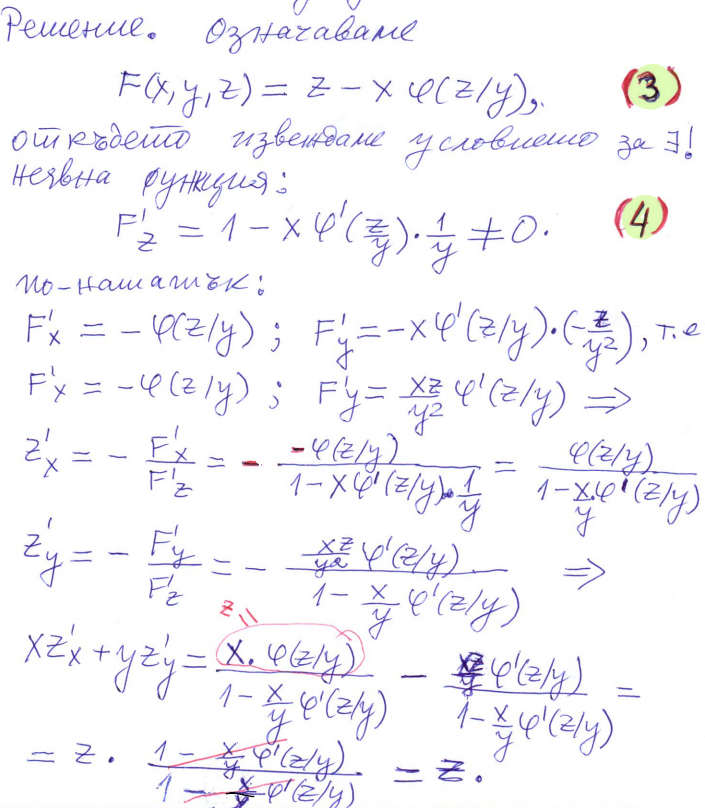
\includegraphics{Pics/calc/ex7-task4.png}
\end{figure}


\newpage
\section{Упражнение към лекция 8}
\subsection{Задачи}

\subsection*{Задача 1}
Да се изследва за локален екстремум следната функция.
$$z = 1-\sqrt{x^2-y^2}$$

\subsection*{Задача 2}
Намерете точките на условен екстремум и екстремумите на следните функции.
\begin{itemize}
\item $z = x^2 + y^2$, aко $x+y=1$
\item $u = x^2 + y^2 - 12x + 16y$, aко $x^2+y^2=25$
\item $u = x + y + z$, ако $z = 1$ и $x^2 + y^2 = 1$
\end{itemize}

\subsection*{Задача 3}
Да се изследва функцията $u = xy + yz$ за условен екстремум, при ограничения.
$$x^2+y^2 = 2$$
$$y+z = 2$$

\subsection*{Задача 4}
Да се изследва функцията $z = x+y$ за условен екстремум, при ограничения.
$$xy = 1$$

\subsection*{Задача 5}
Да се намери дефиниционното множество на функциите.
\begin{itemize}
\item $z = \sqrt{1 - x^2 - y^2 + 2x}$
\item $z = \frac{x^2y}{2x+y}$
\item $z = \arcsin{(x+y)}$
\item $w = \frac{1}{\sqrt{xy}}$
\end{itemize}

\subsection*{Задача 6}
Да се намерят границите ако съществуват.
\begin{itemize}
\item $\lim\limits_{(x,y) \to (0,0)} \frac{\tan(xy)}{xy}$
\item $\lim\limits_{(x,y) \to (0,0)} \frac{y}{\sin{(xy)}}$
\item $\lim\limits_{(x,y) \to (0,0)} \frac{1 - \sqrt{1 - xy}}{xy}$
\end{itemize}

\subsection*{Задача 7}
Да се провери дали уравнението удовлетворява посочената функция.
\begin{itemize}
\item $\frac{\partial^2 z}{\partial x \partial y} = \frac{\partial^2 z}{\partial y \partial z}, z(x,y) = \ln(x^2+y^2+1)$
\item $\frac{x}{y}\frac{\partial z}{\partial x} + \frac{1}{\ln x} \frac{\partial z}{\partial y } = 2z, z(x,y) =x^y$
\item $2 \frac{\partial^2 z}{\partial x^2 } + \frac{\partial^2 z}{\partial x \partial y} = 0, z(x,y) = 2\cos^2(y - \frac{x}{2})$
\item $\frac{\partial u}{\partial x} + \frac{\partial u}{\partial y} + \frac{\partial u}{\partial z} = 1, u(x,y,z) = x + \frac{x-y}{y-z}$
\end{itemize}

\subsection*{Задача 8}
Да се изследват за локален екстремум следните функции.
\begin{itemize}
\item $z = x^4 + y^4- x^2- 2xy - y^2$
\item $z = xy(1 - x - y)$
\item $z = x^3 - y^3 - 3x + 3y + 2$
\item $u = x^3 + y^3 + z^2 - 12xy + 2z$
\end{itemize}

\subsection*{Задача 9}
Да се изследват за локален екстремум следните неявно зададени функции.
\begin{itemize}
\item $x^3 + y^3 = 3xy, y = y(x)$
\item $y^2 -3y - \sin(x)= 0, y = y(x)$
\item $x^2 + y^2 + z^2 - xz -yz + 2x + 2y + 2z - 2 = 0, z = z(x,y)$
\item $2x^2 + 2y^2 + z^2 + 8xz -8yz + 8 = 0, z = z(x,y)$
\end{itemize}

\subsection*{Задача 10}
Да се изследва за условен екстремум
\begin{itemize}
\item $z = xy$, aко $2x+y=1$
\item $z = x^2 + y^2$, aко $x - y =1$
\item $u = x^2 + y^2 + z^2$, ако $\frac{x^2}{16} + \frac{y^2}{9} + \frac{z^2}{4} = 1$
\item $u = xyz$, ако $x + y + z = 5, xy+yz+zx = 8$ 
\end{itemize}

\subsection*{Задача 11}
Намерете точките на условен екстремум и екстремумите на следните функции.
\begin{itemize}
\item $u = x^2 + y^2+ z^2 +2x + 4y -6z $, aко $ x^2 + y^2+ z^2 = 14$
\item $u = x^2 + y^2 + z^2 + 2x + 4y $, ако $x^2 + y^2 = 20$
\item $u = x^2 + y^2+ z^2 +6x - 2y + 4z $, ако $x^2 + y^2+ z^2 = 56$ 
\end{itemize}

\subsection*{Задача 12}
Намерете абсолютните екстремуми на следните функции и определете вида им (условен, локален, минимум, максимум)
\begin{itemize}
\item $u = x^2 + y^2 - 12x + 16y$, aко $ x^2 + y^2 \leq 25, x^2 + y^2 \leq 400, x^2 + y^2 \leq 100$
\item $u = x^2 + y^2+ z^2 +2x + 4y -6 $, ако $x^2 + y^2 + z^2 \leq 9$
\item $u = x^2 + 2y^2+ 3z^2$, ако $x^2 + y^2+ z^2 \leq 100$ 
\end{itemize}

\newpage
\subsection{Решения}
\subsection*{Задача 1}
$$z(\Delta x, \Delta y) - z(0,0) = 1-\sqrt{\Delta x^2 - \Delta y^2} - 1 = -\sqrt{\Delta x^2 - \Delta y^2}< 0$$
Имаме строг локален максимум в $z(0,0) = 1$

\subsection*{Задача 2}

\subsection*{Задача 3}

\subsection*{Задача 4}

\subsection*{Задача 5}

\subsection*{Задача 6}

\subsection*{Задача 7}

\subsection*{Задача 8}

\subsection*{Задача 9}

\subsection*{Задача 10}

\subsection*{Задача 11}

\subsection*{Задача 12}

\newpage 
\section{Упражнение към лекция 9}

\subsection{Задачи}

\subsection*{Задача 1}
Да се пресметнат интегралите
\begin{itemize}
\item $I = \iint\limits_D xy \,dx \,dy$, $D: \begin{cases} 0 \leq x \leq 1 \\ 0 \leq y \leq 2 \end{cases}$
\item $I = \iint\limits _D xy \,dx \,dy$, ако D e oградена от $\begin{cases} xy = 1 \\ x+y = \frac{5}{2} \end{cases}$
\item $I = \iint\limits _D \,dx \,dy$, ако D e оградена от кривите$D: \begin{cases} 4y = x^2 - 4x \\ x - y - 3 = 0 \end{cases}$
\end{itemize}

\subsection*{Задача 2}
Да се определят границите на интегриране и да се пресметне интеграла
$$\iint\limits_D (x^2 + y^2) \, dx \, dy, \qquad D: \begin{cases} y = x , \quad y =2 \\ y = x + 2, \quad y = 6 \end{cases}$$

\subsection*{Задача 3}
Да се пресметне интеграла
$$\iint\limits_D (x+y) \, dx \, dy, \qquad \partial D: \begin{cases} y^2 = 2x \\ x+y = 4 \\ x+y = 12 \end{cases}$$

\subsection*{Задача 4}
Да се пресметне интеграла
$$\iint\limits_D (x+y) \, dx \, dy$$
Където D е триъгълник $\triangle ABO$ с върхове $A(1,0),\, B = (1,1),\, O = (0,0)$

\newpage
\subsection{Решения}

\subsection*{Задача 1}

\subsection*{Задача 2}

\subsection*{Задача 3}

\subsection*{Задача 4}


\newpage 
\section{Упражнение към лекция 10}

\subsection{Задачи}

\newpage
\subsection{Решения}

\newpage 
\section{Упражнение към лекция 11}

\subsection{Задачи}

\newpage
\subsection{Решения}


\end{document}